
%!TEX root = paper.tex

\subsection{Data collection}
Movielens\footnote{www.movielens.org} is a recommender system that utilizes collaborative filtering
algorithms to recommend movies to their users based
on their preferences.
We collected ratings from the Movielens users on certain sets of movies. These
sets were generated by selecting five movies from the movies that user has
already rated. There was no overlap among the sets presented to the user in a
session. The user can rate at most 50 such sets in a session. An example of
the questionnaire eliciting a user's rating on a set of movies is shown in the
Figure~\ref{fig:mlset}. The rating widget in the interface could be rated from 0 to 5 with a
precision of 0.5. For the purpose of data collection, we selected users who were active on the
Movielens since January 2015. The data was gathered from the user's responses to
the questionnaire from Feb 2016 to April 2016.


\begin{figure}[ht]
  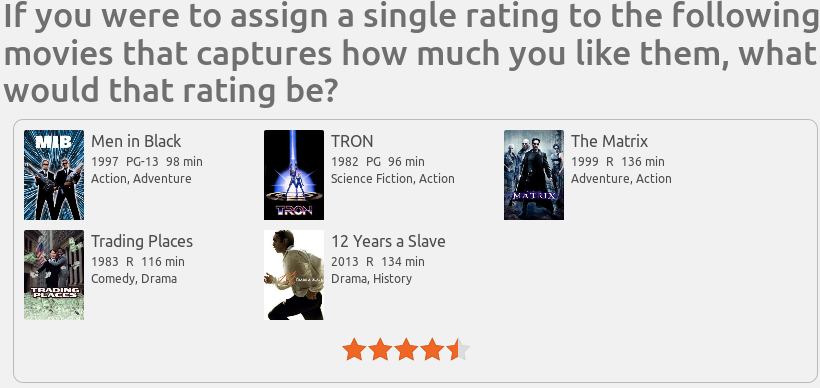
\includegraphics[scale=0.30]{figures/mlset.png}
  \caption{The interface used to elicit users' ratings on a set of movies.}
  \label{fig:mlset}
\end{figure}

\subsection {Data pre-processing}
Before processing the dataset, we removed users who have rated sets within a
time interval of less than one second to avoid users who might be guessing
the ratings at random. 



\subsection{Analysis of set ratings}
After data pre-processing step, we were left with ratings
from 854 users over 29,516  sets containing 12,549 items. 
Figure~\ref{fig:setratingdist} depicts
the distribution of the collected ratings. We also computed the mean rating of
each user and is shown in the Figure~\ref{fig:meanratingdist}.  

\begin{figure}[ht]
  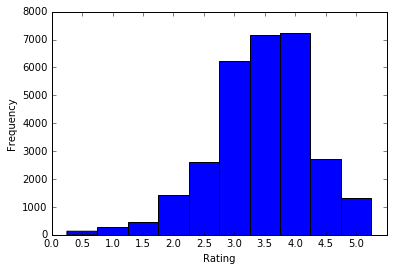
\includegraphics[scale=0.65]{figures/setratingdist.png}
  \caption{Ratings distribution.}
  \label{fig:setratingdist}
\end{figure}

\begin{figure}[ht]
  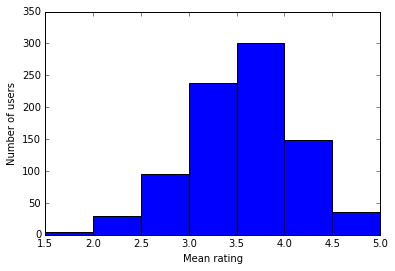
\includegraphics[scale=0.65]{figures/meanratingdist.png}
  \caption{The distribution of users' mean rating.}
  \label{fig:meanratingdist}
\end{figure}



The Figure~\ref{fig:usersetdist} shows the distribution of the number of sets rated by the user,
and we can see that roughly half of the users, i.e., 428 users have rated more
than 90\% of the sets, i.e., at least 45 sets in a session.

\begin{figure}[ht]
  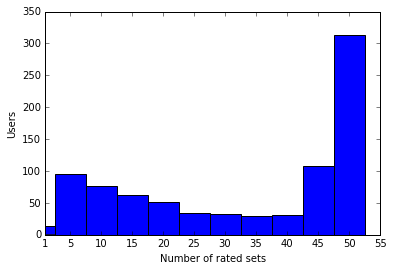
\includegraphics[scale=0.65]{figures/usersetdist.png}
  \caption{The distribution of number of sets rated by the users.}
  \label{fig:usersetdist}
\end{figure}

Since we know the actual rating of the users over the movies in the sets,
these ratings can help us understand the users' behavior when assigning a single
rating to a set of movies. To this end, we computed the deviation of the 
rating assigned by a user to the set
from the average of the user's  ratings of the items constituting the set. To
calculate this deviation we computed the Root Mean Square Error (RMSE) between
the ratings assigned to the sets and the average of the user-item ratings in
the sets. As can be seen in the Table~\ref{table:sets_rmse_table}, this RMSE
over all the sets is 0.597. Subsequently, we looked at the fraction of sets that are
rated below the average of the ratings of the items in the set. We refer to
these sets as the under-rated sets. Similarly, the over-rated sets are
those sets that are rated above the average of the ratings of the items in the
set.We used a margin of 0.5 while identifying these sets, i.e., sets rated
within the margin of 0.5 of their average rating were considered neither as
over-rated or under-rated sets.

%TODO:statistical significance of lower RMSE
The Table~\ref{table:sets_rmse_table} shows that the majority of the sets were neither over-rated or
under-rated and had a significantly lower RMSE of 0.241 when compared against
under-rated or over-rated sets. Further, we selected users who have rated at
least 50 sets and computed the fraction of under-rated and over-rated sets.
As can be seen from the Figure~\ref{fig:underrated}, some users tend to over-rate or under-rate sets
and by the Kolmogorov-Smirnov 2 sample test this behavior was found to be
statistically different (P-value $<$ 1e-16) from that of random.

\begin{table}[t]
  \centering
  \caption{RMSEs across different type of sets.}
  \label{table:sets_rmse_table}
  \begin{tabular}{|l|c|c|c|}
    \hline
    Type
    &\multicolumn{1}{|p{2cm}|}{\centering \% of Sets}
    &\multicolumn{1}{|p{2cm}|}{\centering Number of Sets}
    &\multicolumn{1}{|p{1cm}|}{\centering RMSE} \\
    \hline
    Over-rated  & 17.68 & 5,220  & 0.962 \\
    Under-rated & 22.26 & 6,571  & 0.810 \\
        Neither & 60.05 & 17,725  & 0.241 \\
    \hline
    All & 100   & 29,516 & 0.597 \\
    \hline
  \end{tabular}
\end{table}


\begin{figure*}[ht]
  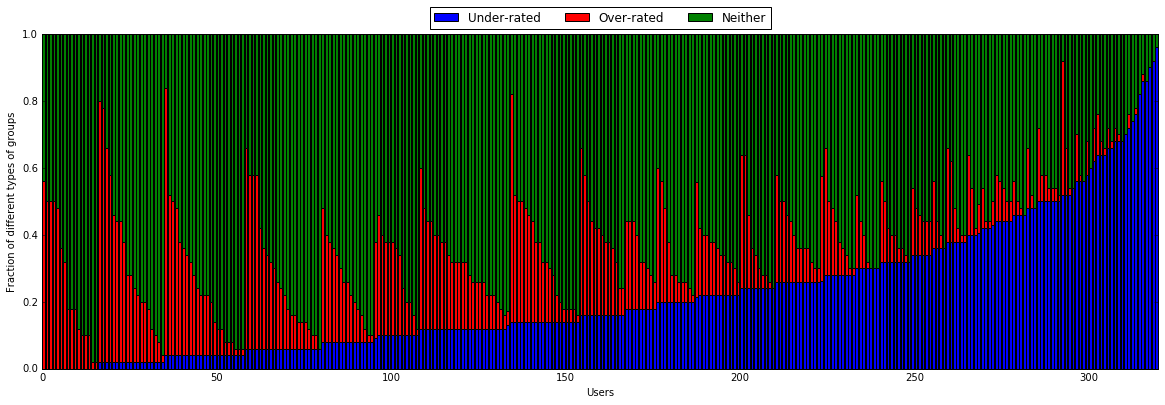
\includegraphics[scale=0.45]{figures/underrated.png}
  \caption{Fraction of different types of sets across users.}
  \label{fig:underrated}
\end{figure*}


Further, we examined the effect of diversity of the items' rating in the set,
i.e., whether the presence of movies with varying degree of ratings has any
effect on the rating assigned by the user to the set. For each set, we
computed the difference between the item's rating and the average of the ratings
in the set. We defined set-deviation as the square root of the mean of this
difference of the items' ratings in the set. The sets having deviation
greater than 1.0 were characterized as "Diverse" sets and rest as
"Non-Diverse" sets. Following this characterization in the dataset, nearly 20\%
of the sets are diverse sets having RMSE of 0.725 while remaining sets
have lower RMSE of 0.559.  This indicates that user seems to under-rate or
over-rate diverse sets more in comparison to non-diverse sets.


We also investigated whether the presence of movies that are rated recently or
that are rated in the past has an effect on the rating assigned to the set.
To this end, for each set we computed the difference between the timestamp of
the earliest rating and 2016, i.e. when the users were asked to rate the sets.
Interestingly, the under-rated sets contained ratings that were provided on
average 1,800 days,i.e., five years before the survey while remaining sets
contained ratings that were provided approximately 1,450 days, i.e.,
four years before the survey. This difference among the sets was found to be
statistically significant by T-test, i.e. P-value $<$ 1e-16. This suggests that
the user's preference for a movie in a set appears to decay temporally leading
to under-rating of the set containing that movie.

